\documentclass[tikz,border=8pt]{standalone}
\usepackage[T1]{fontenc}
\usepackage[utf8]{inputenc}
\usepackage{amsmath}
\usepackage{xcolor}
\usetikzlibrary{arrows.meta,calc,decorations.pathreplacing,positioning}

\definecolor{itblue}{RGB}{40,86,135}
\definecolor{itlightblue}{RGB}{229,239,249}
\definecolor{itgreen}{RGB}{30,128,92}
\definecolor{itlightgreen}{RGB}{226,244,236}
\definecolor{itorange}{RGB}{232,126,32}
\definecolor{itlightorange}{RGB}{255,235,209}
\definecolor{itgray}{RGB}{92,99,112}

\begin{document}
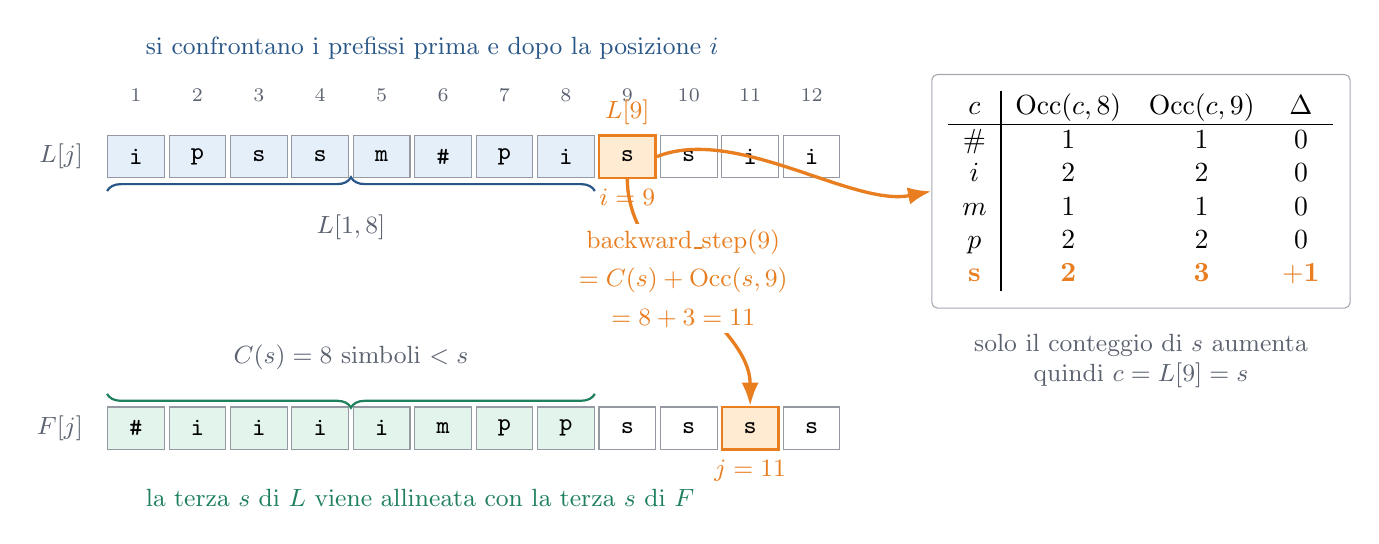
\begin{tikzpicture}[
    >=Latex,
    cell/.style={
        draw=itgray!65,
        minimum width=0.72cm,
        minimum height=0.54cm,
        inner sep=0pt,
        font=\small\ttfamily
    },
    index/.style={font=\scriptsize, text=itgray},
    label/.style={font=\small, text=itgray},
    note/.style={font=\small, align=center},
    arrow/.style={->, very thick, itorange}
]

% L row.
\node[label, anchor=east] at (-0.55,0) {$L[j]$};
\foreach \j/\ch in {1/i,2/p,3/s,4/s,5/m,6/\#,7/p,8/i,9/s,10/s,11/i,12/i} {
    \pgfmathsetmacro{\x}{0.78*(\j-1)}
    \node[index] at (\x,0.78) {\j};
    \ifnum\j<9
        \node[cell, fill=itlightblue] (L\j) at (\x,0) {\ch};
    \else
        \ifnum\j=9
            \node[cell, fill=itlightorange, draw=itorange, line width=0.9pt] (L\j) at (\x,0) {\textbf{\ch}};
        \else
            \node[cell, fill=white] (L\j) at (\x,0) {\ch};
        \fi
    \fi
}
\draw[decorate, decoration={brace, amplitude=5pt}, itblue, thick]
    ($(L1.south west)+(0,-0.16)$) -- ($(L8.south east)+(0,-0.16)$)
    node[midway, below=5pt, label] {$L[1,8]$};
\node[note, text=itorange, anchor=north] at (L9.south) {$i=9$};
\node[note, text=itorange, anchor=south] at (L9.north) {$L[9]$};

% Occ table.
\node[anchor=north west, draw=itgray!55, fill=white, rounded corners=2pt, inner sep=6pt] (occ) at (10.1,1.05) {
    $\begin{array}{c|ccc}
        c & \operatorname{Occ}(c,8) & \operatorname{Occ}(c,9) & \Delta \\
        \hline
        \# & 1 & 1 & 0 \\
        i  & 2 & 2 & 0 \\
        m  & 1 & 1 & 0 \\
        p  & 2 & 2 & 0 \\
        \color{itorange}{\mathbf{s}} & \color{itorange}{\mathbf{2}} & \color{itorange}{\mathbf{3}} & \color{itorange}{\mathbf{+1}}
    \end{array}$
};
\node[note, text=itgray, below=2mm of occ] (onlys)
    {solo il conteggio di $s$ aumenta\\ quindi $c=L[9]=s$};
\draw[arrow] (L9.east) .. controls +(1.0,0.4) and +(-1.0,-0.2) .. (occ.west);

% F row.
\node[label, anchor=east] at (-0.55,-3.45) {$F[j]$};
\foreach \j/\ch in {1/\#,2/i,3/i,4/i,5/i,6/m,7/p,8/p,9/s,10/s,11/s,12/s} {
    \pgfmathsetmacro{\x}{0.78*(\j-1)}
    \ifnum\j<9
        \node[cell, fill=itlightgreen] (F\j) at (\x,-3.45) {\ch};
    \else
        \ifnum\j=11
            \node[cell, fill=itlightorange, draw=itorange, line width=0.9pt] (F\j) at (\x,-3.45) {\textbf{\ch}};
        \else
            \node[cell, fill=white] (F\j) at (\x,-3.45) {\ch};
        \fi
    \fi
}
\draw[decorate, decoration={brace, mirror, amplitude=5pt}, itgreen, thick]
    ($(F1.north west)+(0,0.16)$) -- ($(F8.north east)+(0,0.16)$)
    node[midway, above=5pt, label] {$C(s)=8$ simboli $<s$};
\node[note, text=itorange, anchor=north] at (F11.south) {$j=11$};

% LF explanation.
\draw[arrow] (L9.south) .. controls +(0,-1.15) and +(0,1.05) .. (F11.north);
\node[note, fill=white, inner sep=2pt, text=itorange] at (6.95,-1.55)
    {$\operatorname{backward\_step}(9)$\\[1mm]
     $=C(s)+\operatorname{Occ}(s,9)$\\[1mm]
     $=8+3=11$};

\node[note, text=itblue, anchor=west] at (0.0,1.38)
    {si confrontano i prefissi prima e dopo la posizione $i$};
\node[note, text=itgreen, anchor=west] at (0.0,-4.33)
    {la terza $s$ di $L$ viene allineata con la terza $s$ di $F$};

\end{tikzpicture}
\end{document}
